\documentclass{scrartcl}

\usepackage[utf8]{inputenc}
\usepackage[T1]{fontenc}
\usepackage{lmodern}
\usepackage{babel}
\usepackage{amsmath}
\usepackage{amsthm}
\usepackage{mathtools}
\usepackage[dvipsnames]{xcolor}
\usepackage{tikz}
\usepackage{pgfplots}
\usepackage{amssymb}
\usepackage{enumitem}
\usepackage{import}

\subimport{docs/libs/}{init}

\usetikzlibrary{positioning}


\usepackage[
backend=biber,
% style=alphabetic,
sorting=none
]{biblatex}

\addbibresource{whitepaper.bib}

\title{Rule based Symbolic Reasoning}
\author{Matthias Lochbrunner}
\date{\today}

\theoremstyle{definition}
\newtheorem{exmp}{Example}[section]

\pgfplotsset{colormap/jet}

\tikzset{
    fromColorBar/.style={
        color of colormap={1000-#1*10},
        fill=.,
    },
}

\begin{document}
\maketitle
\begin{center}
	\textbf{Abstract}
\end{center}
\begin{abstract}
	The combination of a rule based beam search and deep learning is a promising approach to solve mathematical problems.
	One obstacle to overcome is the amount of possible branches in this search as the number of applicable rules and length of the calculation increases.
	This paper proposes to address this issue by constantly shrinking the beam size with a multi-head neuronal network:
	A policy head selects rules and positions in the current term.
	A value head evaluates the probability that this calculation could lead to the desired solution.
	Both heads help to reduce the beam size such that solving advanced mathematical problems becomes feasible.
\end{abstract}

\section{Motivation}

Since current approaches to solve mathematical problems use a complex but fixed set of rules, it takes manual effort to extend their capabilities \cite{wolfram}.
The generic approach described here might be able to incorporate additional rules without requiring manual work.
Moreover, it is not limited to mathematical calculus as long as the domain can be described by a well-defined, human-readable rule set.
The correctness of the result depends only on the correctness of the given rule set.

\section{Related work}

\begin{itemize}
	\item Lampe et. al. use state of the art sequence to sequence transformers on polish notation formatted equations \cite{Lample2020Deep}.
	This approach sees solving of a mathematical problem as a translation problem on 1d data.
	They don't use the concept of rules and tree structured data in the network.
	\item Todo: Find more related work.
\end{itemize}

\section{Method}

Given a problem, e.g. solve the equation $T_1\left(x\right)\equiv T_2\left(x\right)$ for $x$,
the beam search could try to apply various rules at different nodes in the syntax tree of the equation.
The policy head proposes the most promising combination of rules and positions in the current equation.
The value head evaluates the probability of success of the current calculation step.
The cumulative result of the value head can abort the solution path of the attempt, as it "seems" unlikely that the this attempt could succeed \cite{44806}.

\subsection{Rule Application}

Every rule is of the shape $A \Longrightarrow B$ or $A \equiv B$, which is equivalent to $A \Longleftrightarrow B$ or just the combination of $A \Longrightarrow B$ and $B \Longrightarrow A$.
Without loss of correctness we just use the first shape $A \Longrightarrow B$ in this paper.
Let's name the term $T\left(x\right)$ with the depth $d$ of the corresponding syntax tree representation.
As the term can be represented by a tree we will name it's child terms $T_p$ with the position $p \in \big\{\left( n_1, n_2, \dots, n_d \right) : n_i \in \mathbb{N}, n_i \leq s \big\}$.
The root symbol of $T_p$ should be $t_p$.
Hence the sub-terms of $T$ be $T_p$ where $T_1$ for instance is the first child node of the root in that tree and $T_{1,1}$ the first child of $T_1$ and so on.
Let $s$ be the maximal number of children per node in the syntax tree.

We try to match condition $A$ of a rule at any position $p$ of term $T\left(x\right)$.
Doing so results in a list of possible positions $p_j$ with the required substitution table $M_j: S_A \to S_{T_p}$,
where $S_{T_p} \equiv \big\{ t_q : \forall q \text{ below } p\big\}$ is the set of the symbols in term $T_p$ and $S_A$ the set of symbols in the condition $A$.
Then the application of that rule results in the new terms $T^{(j)}$ where each node at $p_j$ gets replaced by the modified conclusion $B'^{(j)} \coloneqq M_j\left( B \right)$.
Where $B'^{(j)}$ is $B$ with symbols mapped back by by $M_j$. 

\begin{exmp}
To illustrate the above, let's look at the application of the derivative rule for polynomials.
% TODO: Add connection example <-> theoretcih

Consider the derivative rule
\begin{align}
	\frac{\partial}{\partial {\color{red}x}} {\color{red}x}^{\color{blue}n} \Longrightarrow {\color{blue}n}\cdot {\color{red}x}^{{\color{blue}n}-1} 
\end{align}
applied to the term
\begin{align}
	\frac{\partial}{\partial {\color{red}z}} {\color{red}z}^{\color{blue}4}
\end{align}.
Using the symbolic mapping $M\left({\color{red}x}\right) = \color{red}z$ and $M\left({\color{blue}n} \right) = {\color{blue}4}$ leads to the new term
\begin{align}
	{\color{blue}4}\cdot {\color{red}z}^{{\color{blue}4}-1} 
\end{align}.

\end{exmp}

\subsection{Network Architecture for Tree Structured Data}

Lampe et. al. showed an approach where they unroll the term $T$ using the polish notation.
Then they apply contemporary NLP translation methods on the that sequence where the resulting "translated sentence" is the next step in the calculation. \cite{Lample2020Deep}
The approach discussed here keeps the tree structure. It turned out that Tree-LSTM perform poorly on that data \cite{tai2015improved}.

% network picture

This paper will discuss the adoption of two different architectures:
Indexed convolution and attention networks with special positional encoding.

\subsubsection{Indexed Convolution}

The indexed CNN operation performs a convolution of each node on it's neighbor nodes and itself.
In order to increase the compute efficiency each term is rolled out.
Let $t_p$ be the symbol at the root of sub-term $T_p$,
then the breadth-first unrolled tern with $s=2$ is the vector $\left( t, t_1, t_1, t_{1,1},t_{1,2}, t_{2,1}, t_{2,2}, \cdots \right)$ with length $L$.
An index map $g \in \mathbb{N}^{\ell\times \left( s+2 \right)}$ carries the index of the neighbors in a constant order.


\begin{figure}[!htbp]
	\centering
	\def\ConvColor{rgb:yellow,5;red,2.5;white,5}
\def\ConvReluColor{rgb:yellow,5;red,5;white,5}

% keine batch
\begin{tikzpicture}
\tikzstyle{connection}=[ultra thick,every node/.style={sloped,allow upside down},draw=\edgecolor,opacity=0.7]

\pic[shift={(0,0,0)}] at (0,0,0) {RightBandedBox={name=ix,caption=x,%
        xlabel={{"t", "f"}},ylabel=L,zlabel=b,fill=\ConvColor,bandfill=\ConvColor,%
        height=8,width={2, 3},depth=8}};

\pic[shift={(0,3,0)}] at (0,0,0) {Box={name=i1,caption=g,%
        xlabel={{"2+s"}},ylabel=L,zlabel=b,fill=\ConvColor,%
        height=8,width={2},depth=8}};

\pic[shift={(2,0,0)}] at (ix-east) {RightBandedBox={name=ic1,caption=iconv,%
        xlabel={{"e"}},ylabel=L,zlabel=b,fill=\ConvColor,bandfill=\ConvReluColor,%
        height=10,width={3},depth=10}};

\pic[shift={(4,0,0)}] at (ix-east) {RightBandedBox={name=ic2,caption=iconv,%
        xlabel={{"e"}},ylabel=L,zlabel=b,fill=\ConvColor,bandfill=\ConvReluColor,%
        height=10,width={3},depth=10}};

% heads

\pic[shift={(8,0,-4)}] at (ix-east) {RightBandedBox={name=icv,caption=iconv,%
xlabel={{"e"}},ylabel=L,zlabel=b,fill=\ConvColor,bandfill=\ConvReluColor,%
height=10,width={3},depth=10}};

\pic[shift={(10,0,-4)}] at (ix-east) {Box={name=ov,caption=value,%
xlabel={{"1"}},zlabel=b,ylabel=1,fill=\ConvColor,%
height=1,width={1},depth=10}};

\pic[shift={(8,0,4)}] at (ix-east) {RightBandedBox={name=icp,caption=iconv,%
        xlabel={{"e", "dummy"}},ylabel=L,zlabel=b,fill=\ConvColor,bandfill=\ConvReluColor,%
        height=10,width={3},depth=10}};

\pic[shift={(10,0,4)}] at (ix-east) {Box={name=op,caption=policy,%
        xlabel={{"r", "dummy"}},ylabel=L,zlabel=b,fill=\ConvColor,%
        height=10,width={8},depth=10}};


\path (ix-east) -- (ix-west) coordinate[pos=0.4] (after4) ;

\draw [connection] (ix-east) -- node {\midarrow} (ic1-west);
\draw [connection]  (ic1-east) -- node {\midarrow} (ic2-west);
\draw [connection]  (ic2-east) -- node {\midarrow} (icv-west);
\draw [connection]  (icv-east) -- node {\midarrow} (ov-west);
\draw [connection]  (ic2-east) -- node {\midarrow} (icp-west);
\draw [connection]  (icp-east) -- node {\midarrow} (op-west);

\draw [connection] (i1-east) -- ++ (2.5,0,0) -- node {\midarrow} (ic1-west);
\draw [connection] (i1-east) -- ++ (4.5,0,0) -- node {\midarrow} (ic2-west);
\draw [connection] (i1-east) -- ++ (5,0,0) -- ++ (3.5, 0, -4) -- node {\midarrow} (icv-west);
\draw [connection] (i1-east) -- ++ (5,0,0) -- ++ (3.5, 0, +4) -- node {\midarrow} (icp-west);

\end{tikzpicture}

	\caption{The index tensor is an additional input of this network architecture.
		Each indexed convolution operations reads from that index tensor.
		The policy head returns for each sample a matrix of with the axis rule id and path id. 
		The output of the value head is one scalar per sample in the mini-batch. 
	}
	\label{fig:iconv_network}
\end{figure}

% Was geht rein und was geht raus
With the input channel size $i$ and output channel size $j$, the kernel weights $w \in \mathbb{R}^{\left( s+2 \right)\times i \times j}$ and bias $b \in \mathbb{R}^j$,
the indexed convolution $C$ is defined as

\begin{align}
	C\left( x, g, w, b \right)_{\ell j} \coloneqq \sum_{ki}x_{g_{\ell k}i} w_{kij}+b_j
\end{align}

where $1 \leq \ell \leq L$ is the index of symbol $t_p$ in the unrolled term. Figure \ref{fig:iconv_network}


\begin{figure}[!htbp]
	\centering
	
% sample id: #19818
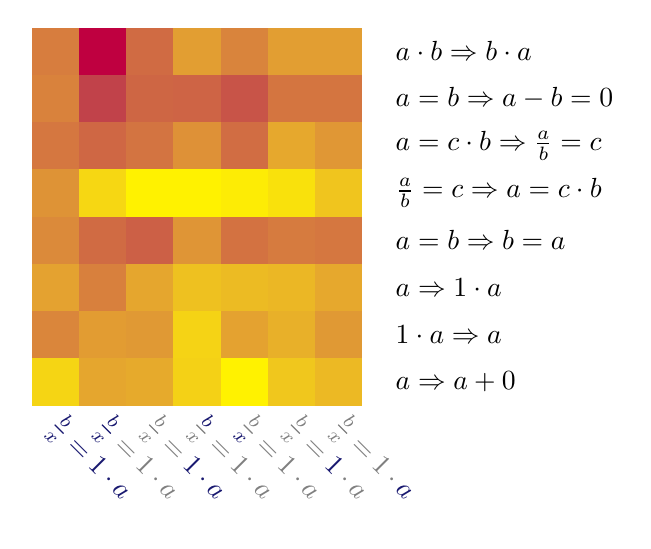
\begin{tikzpicture}[scale=0.6]
    \foreach \y [count=\p] in {
        {40,0,30,58,44,58,58},
        {43,6,27,26,17,36,36},
        {37,28,35,51,31,63,54},
        {52,87,100,100,97,92,78},
        {47,30,24,53,34,39,37},
        {60,42,62,76,73,71,63},
        {45,57,55,85,60,67,55},
        {86,62,64,84,100,79,72},
        } {
        \foreach \x [count=\r] in \y {
            \node[fill=yellow!\x!purple, minimum size=6mm, text=white] at (\r,-\p) {};
        }
    }
    \foreach \t [count=\p] in {
        $a\cdot b \Rightarrow b\cdot a $,
        $a=b \Rightarrow a-b=0 $,
        $a=c\cdot b \Rightarrow \frac{a}{b}=c $,
        $\frac{a}{b}=c \Rightarrow a=c\cdot b $,
        $a=b \Rightarrow b=a $,
        $a \Rightarrow 1\cdot a $,
        $1\cdot a \Rightarrow a $,
        $a \Rightarrow a+0 $
    } {
        \node[anchor=west] at (8, -\p) {\t};
    }
    \foreach \t [count=\r] in {
        $\textcolor{MidnightBlue}{\frac{b}{x}=1\cdot a}$,
        $\textcolor{Gray}{\textcolor{MidnightBlue}{\frac{b}{x}}=1\cdot a}$,
        $\textcolor{Gray}{\frac{b}{x}=\textcolor{MidnightBlue}{1\cdot a}}$,
        $\textcolor{Gray}{\frac{\textcolor{MidnightBlue}{b}}{x}=1\cdot a}$,
        $\textcolor{Gray}{\frac{b}{\textcolor{MidnightBlue}{x}}=1\cdot a}$,
        $\textcolor{Gray}{\frac{b}{x}=\textcolor{MidnightBlue}{1}\cdot a}$,
        $\textcolor{Gray}{\frac{b}{x}=1\cdot \textcolor{MidnightBlue}{a}}$
    } {
        \node[anchor=west, rotate=-45] at (\r - 0.2, -8.7) {\t};
    }
    \end{tikzpicture}
    
	\caption{Policy Network output: Each row is a possible rule. Each column a sub-term $T_{p_j}$ of the initial term $T$ (highlighted in blue).
	Rules which are not applicable for the any $T_{p_j}$ are not shown here.
	This heat-map shows that dividing the equation by $a$ is more promising than blowing it up with the rules in in the in the at the bottom of the map.}
	\label{fig:network_output}
\end{figure}

Figure \ref{fig:network_output} demonstrates the output of the policy head applied on the term $\frac{b}{x}=1\cdot a$ .

\subsubsection{Transformer and Positional Encoding}

Positional encoding $PE\left( pos\right)$ in NLP is used to "attach" the position $pos$ of a word in the sentence to the embedding of that word \cite{vaswani2017attention}.
The desired properties for the positional encoding sub-terms $T_a$ and $T_b$ should be:
\begin{enumerate}[label=(\roman*)]
	\item $PE\left( T_a \right) - PE\left( T_a \right)$ is metric for the relative position of sub-terms $T_A$ and $T_B$.
	\item $PE\left( T_a \right) - PE\left( T_a \right)$ is independent of the absolute position of the sub-terms.
\end{enumerate}

A naive approach is to draw the tree on a two dimensional plane and count the sub-terms from left to right.
This approach does not fullfil any of the desired properties.

But dividing these numbers iteratively by the spread $s$.

\begin{align}
	PE^{(n+1)}\left( T \right) \coloneqq \lfloor \frac{PE^{(n)} \left( T \right)}{s} \rfloor
\end{align}

the collection of $PE^{(n+1)}\left( T \right)$ partly fulfills these properties.
This could be good enough as input for sine and cosine functions or learnable embeddings \cite{gehring2017convolutional}.


\subsection{Three-T-Loop}

The training set consists of problems generated with sympy. \cite{10.7717/peerj-cs.103}.
A training sample also has the shape of a rule $T^{(\text I)} \Longrightarrow T^{(\text T)}$ where $T^{(\text I)}$ is the starting point and $T^{(\text T)}$ the solution term.
The goal is to find the shortest chain of rule application that lead to the target term:

\begin{align}
	T^{(\text I)} \Longrightarrow T^{(j_1)} \Longrightarrow T^{(j_1j_2)} \Longrightarrow \cdots \Longrightarrow T^{(\text T)}
	\label{eq:calculation_chain}
\end{align}

To obtain trainable data from the given problem set, we use an initial beam search without the assistance of a network.
A few simple problems can already be solved and learnable data can be extracted from these solution paths.
Let's call this procedure \textit{three-T-loop} which consists of these three steps:

\begin{enumerate}[label=(\roman*)]
	\item \textbf{Try} to solve some of the training problems.
	\item \textbf{Trace} the calculation steps of the solved problems and create training data out of them.
	\item \textbf{Train} the model with the trainings data from the previous step.
\end{enumerate}

In each iteration of that \textit{three-T-loop} the number of trainable data increases. 
As the network's performance increases, it can solve more and more problems.
The trained network also reduces the amount of used rule applications as they are cancelled depending on the outcome of the value head (see Figure \ref{fig:beam_search} on page \pageref{fig:beam_search}). 


This loop can be extended by a forth step discussed in the outlook section, which allows to incorporate useful sub chains of formula (\ref{eq:calculation_chain}) into the rule set.

\begin{figure}[!htbp]
	\centering
	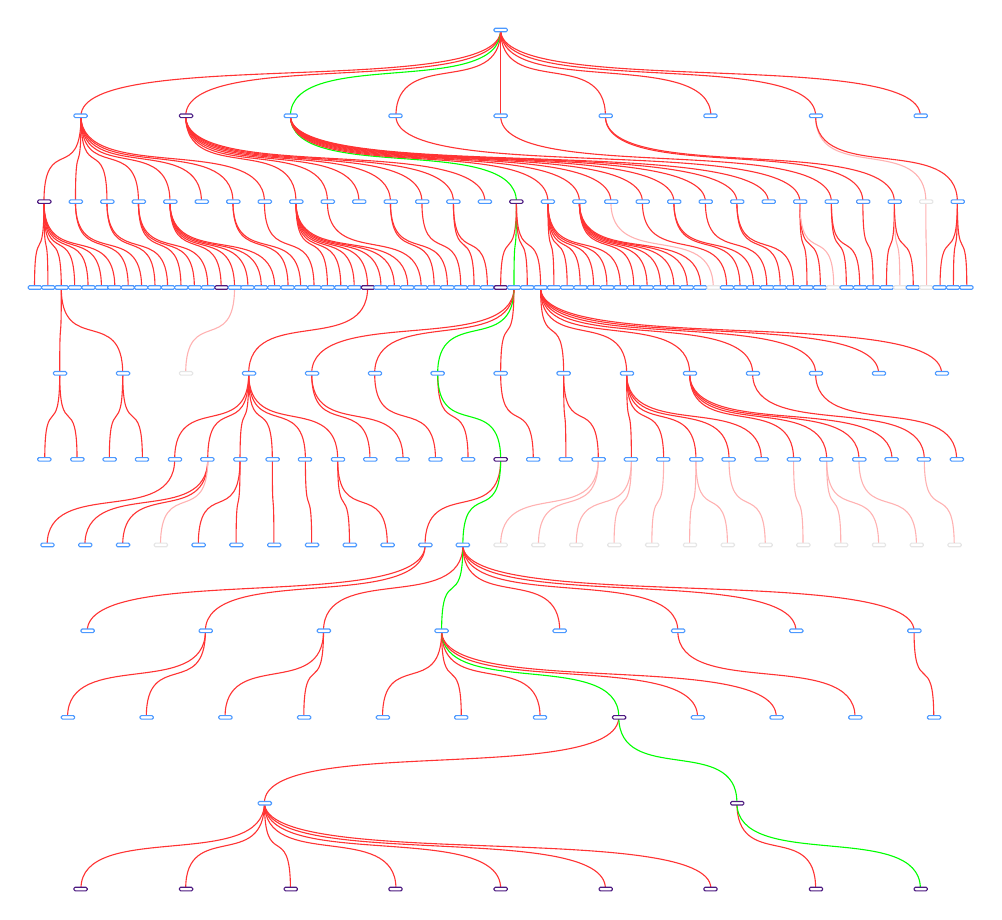
\begin{tikzpicture}[every node/.style={rectangle,fill=white,rounded corners=0.451}]
	\tikzset{xcolor/.code args={#1=#2}{
		\definecolor{mytemp}{rgb}{#2}
		\tikzset{draw=mytemp}
		}
	}
	\fontsize{0.5634}{0.6761}\selectfont
	\draw[draw=red!80] (-5.33,4.36) .. controls (-5.33,5.24) and (0.00,4.58) .. (0.00,5.45);
	\draw[draw=red!80] (-5.80,3.27) .. controls (-5.80,4.15) and (-5.33,3.49) .. (-5.33,4.36);
	\draw[draw=red!80] (-5.92,2.18) .. controls (-5.92,3.05) and (-5.80,2.40) .. (-5.80,3.27);
	\draw[draw=red!80] (-5.75,2.18) .. controls (-5.75,3.05) and (-5.80,2.40) .. (-5.80,3.27);
	\draw[draw=red!80] (-5.58,2.18) .. controls (-5.58,3.05) and (-5.80,2.40) .. (-5.80,3.27);
	\draw[draw=red!80] (-5.60,1.09) .. controls (-5.60,1.96) and (-5.58,1.31) .. (-5.58,2.18);
	\draw[draw=red!80] (-5.79,-8.88e-16) .. controls (-5.79,0.873) and (-5.60,0.218) .. (-5.60,1.09);
	\draw[draw=red!80] (-5.38,-8.88e-16) .. controls (-5.38,0.873) and (-5.60,0.218) .. (-5.60,1.09);
	\draw[draw=red!80] (-4.80,1.09) .. controls (-4.80,1.96) and (-5.58,1.31) .. (-5.58,2.18);
	\draw[draw=red!80] (-4.97,-8.88e-16) .. controls (-4.97,0.873) and (-4.80,0.218) .. (-4.80,1.09);
	\draw[draw=red!80] (-4.55,-8.88e-16) .. controls (-4.55,0.873) and (-4.80,0.218) .. (-4.80,1.09);
	\draw[draw=red!80] (-5.41,2.18) .. controls (-5.41,3.05) and (-5.80,2.40) .. (-5.80,3.27);
	\draw[draw=red!80] (-5.24,2.18) .. controls (-5.24,3.05) and (-5.80,2.40) .. (-5.80,3.27);
	\draw[draw=red!80] (-5.07,2.18) .. controls (-5.07,3.05) and (-5.80,2.40) .. (-5.80,3.27);
	\draw[draw=red!80] (-4.90,2.18) .. controls (-4.90,3.05) and (-5.80,2.40) .. (-5.80,3.27);
	\draw[draw=red!80] (-5.40,3.27) .. controls (-5.40,4.15) and (-5.33,3.49) .. (-5.33,4.36);
	\draw[draw=red!80] (-4.73,2.18) .. controls (-4.73,3.05) and (-5.40,2.40) .. (-5.40,3.27);
	\draw[draw=red!80] (-4.56,2.18) .. controls (-4.56,3.05) and (-5.40,2.40) .. (-5.40,3.27);
	\draw[draw=red!80] (-5.00,3.27) .. controls (-5.00,4.15) and (-5.33,3.49) .. (-5.33,4.36);
	\draw[draw=red!80] (-4.39,2.18) .. controls (-4.39,3.05) and (-5.00,2.40) .. (-5.00,3.27);
	\draw[draw=red!80] (-4.23,2.18) .. controls (-4.23,3.05) and (-5.00,2.40) .. (-5.00,3.27);
	\draw[draw=red!80] (-4.60,3.27) .. controls (-4.60,4.15) and (-5.33,3.49) .. (-5.33,4.36);
	\draw[draw=red!80] (-4.06,2.18) .. controls (-4.06,3.05) and (-4.60,2.40) .. (-4.60,3.27);
	\draw[draw=red!80] (-3.89,2.18) .. controls (-3.89,3.05) and (-4.60,2.40) .. (-4.60,3.27);
	\draw[draw=red!80] (-3.72,2.18) .. controls (-3.72,3.05) and (-4.60,2.40) .. (-4.60,3.27);
	\draw[draw=red!80] (-4.20,3.27) .. controls (-4.20,4.15) and (-5.33,3.49) .. (-5.33,4.36);
	\draw[draw=red!80] (-3.55,2.18) .. controls (-3.55,3.05) and (-4.20,2.40) .. (-4.20,3.27);
	\draw[draw=red!80] (-3.38,2.18) .. controls (-3.38,3.05) and (-4.20,2.40) .. (-4.20,3.27);
	\draw[draw=red!30] (-4.00,1.09) .. controls (-4.00,1.96) and (-3.38,1.31) .. (-3.38,2.18);
	\draw[draw=red!80] (-3.21,2.18) .. controls (-3.21,3.05) and (-4.20,2.40) .. (-4.20,3.27);
	\draw[draw=red!80] (-3.04,2.18) .. controls (-3.04,3.05) and (-4.20,2.40) .. (-4.20,3.27);
	\draw[draw=red!80] (-2.87,2.18) .. controls (-2.87,3.05) and (-4.20,2.40) .. (-4.20,3.27);
	\draw[draw=red!80] (-3.80,3.27) .. controls (-3.80,4.15) and (-5.33,3.49) .. (-5.33,4.36);
	\draw[draw=red!80] (-3.40,3.27) .. controls (-3.40,4.15) and (-5.33,3.49) .. (-5.33,4.36);
	\draw[draw=red!80] (-2.70,2.18) .. controls (-2.70,3.05) and (-3.40,2.40) .. (-3.40,3.27);
	\draw[draw=red!80] (-2.54,2.18) .. controls (-2.54,3.05) and (-3.40,2.40) .. (-3.40,3.27);
	\draw[draw=red!80] (-3.00,3.27) .. controls (-3.00,4.15) and (-5.33,3.49) .. (-5.33,4.36);
	\draw[draw=red!80] (-2.37,2.18) .. controls (-2.37,3.05) and (-3.00,2.40) .. (-3.00,3.27);
	\draw[draw=red!80] (-4.00,4.36) .. controls (-4.00,5.24) and (0.00,4.58) .. (0.00,5.45);
	\draw[draw=red!80] (-2.60,3.27) .. controls (-2.60,4.15) and (-4.00,3.49) .. (-4.00,4.36);
	\draw[draw=red!80] (-2.20,2.18) .. controls (-2.20,3.05) and (-2.60,2.40) .. (-2.60,3.27);
	\draw[draw=red!80] (-2.03,2.18) .. controls (-2.03,3.05) and (-2.60,2.40) .. (-2.60,3.27);
	\draw[draw=red!80] (-1.86,2.18) .. controls (-1.86,3.05) and (-2.60,2.40) .. (-2.60,3.27);
	\draw[draw=red!80] (-1.69,2.18) .. controls (-1.69,3.05) and (-2.60,2.40) .. (-2.60,3.27);
	\draw[draw=red!80] (-3.20,1.09) .. controls (-3.20,1.96) and (-1.69,1.31) .. (-1.69,2.18);
	\draw[draw=red!80] (-4.14,-8.88e-16) .. controls (-4.14,0.873) and (-3.20,0.218) .. (-3.20,1.09);
	\draw[draw=red!80] (-5.76,-1.09) .. controls (-5.76,-0.218) and (-4.14,-0.873) .. (-4.14,-8.88e-16);
	\draw[draw=red!80] (-3.72,-8.88e-16) .. controls (-3.72,0.873) and (-3.20,0.218) .. (-3.20,1.09);
	\draw[draw=red!80] (-5.28,-1.09) .. controls (-5.28,-0.218) and (-3.72,-0.873) .. (-3.72,-8.88e-16);
	\draw[draw=red!80] (-4.80,-1.09) .. controls (-4.80,-0.218) and (-3.72,-0.873) .. (-3.72,-8.88e-16);
	\draw[draw=red!30] (-4.32,-1.09) .. controls (-4.32,-0.218) and (-3.72,-0.873) .. (-3.72,-8.88e-16);
	\draw[draw=red!80] (-3.31,-8.88e-16) .. controls (-3.31,0.873) and (-3.20,0.218) .. (-3.20,1.09);
	\draw[draw=red!80] (-3.84,-1.09) .. controls (-3.84,-0.218) and (-3.31,-0.873) .. (-3.31,-8.88e-16);
	\draw[draw=red!80] (-3.36,-1.09) .. controls (-3.36,-0.218) and (-3.31,-0.873) .. (-3.31,-8.88e-16);
	\draw[draw=red!80] (-2.90,-8.88e-16) .. controls (-2.90,0.873) and (-3.20,0.218) .. (-3.20,1.09);
	\draw[draw=red!80] (-2.88,-1.09) .. controls (-2.88,-0.218) and (-2.90,-0.873) .. (-2.90,-8.88e-16);
	\draw[draw=red!80] (-2.48,-8.88e-16) .. controls (-2.48,0.873) and (-3.20,0.218) .. (-3.20,1.09);
	\draw[draw=red!80] (-2.40,-1.09) .. controls (-2.40,-0.218) and (-2.48,-0.873) .. (-2.48,-8.88e-16);
	\draw[draw=red!80] (-2.07,-8.88e-16) .. controls (-2.07,0.873) and (-3.20,0.218) .. (-3.20,1.09);
	\draw[draw=red!80] (-1.92,-1.09) .. controls (-1.92,-0.218) and (-2.07,-0.873) .. (-2.07,-8.88e-16);
	\draw[draw=red!80] (-1.44,-1.09) .. controls (-1.44,-0.218) and (-2.07,-0.873) .. (-2.07,-8.88e-16);
	\draw[draw=red!80] (-1.52,2.18) .. controls (-1.52,3.05) and (-2.60,2.40) .. (-2.60,3.27);
	\draw[draw=red!80] (-1.35,2.18) .. controls (-1.35,3.05) and (-2.60,2.40) .. (-2.60,3.27);
	\draw[draw=red!80] (-1.18,2.18) .. controls (-1.18,3.05) and (-2.60,2.40) .. (-2.60,3.27);
	\draw[draw=red!80] (-2.20,3.27) .. controls (-2.20,4.15) and (-4.00,3.49) .. (-4.00,4.36);
	\draw[draw=red!80] (-1.01,2.18) .. controls (-1.01,3.05) and (-2.20,2.40) .. (-2.20,3.27);
	\draw[draw=red!80] (-1.80,3.27) .. controls (-1.80,4.15) and (-4.00,3.49) .. (-4.00,4.36);
	\draw[draw=red!80] (-1.40,3.27) .. controls (-1.40,4.15) and (-4.00,3.49) .. (-4.00,4.36);
	\draw[draw=red!80] (-0.845,2.18) .. controls (-0.845,3.05) and (-1.40,2.40) .. (-1.40,3.27);
	\draw[draw=red!80] (-0.676,2.18) .. controls (-0.676,3.05) and (-1.40,2.40) .. (-1.40,3.27);
	\draw[draw=red!80] (-1.00,3.27) .. controls (-1.00,4.15) and (-4.00,3.49) .. (-4.00,4.36);
	\draw[draw=red!80] (-0.507,2.18) .. controls (-0.507,3.05) and (-1.00,2.40) .. (-1.00,3.27);
	\draw[draw=red!80] (-0.600,3.27) .. controls (-0.600,4.15) and (-4.00,3.49) .. (-4.00,4.36);
	\draw[draw=red!80] (-0.338,2.18) .. controls (-0.338,3.05) and (-0.600,2.40) .. (-0.600,3.27);
	\draw[draw=red!80] (-0.169,2.18) .. controls (-0.169,3.05) and (-0.600,2.40) .. (-0.600,3.27);
	\draw[draw=red!80] (-0.200,3.27) .. controls (-0.200,4.15) and (-4.00,3.49) .. (-4.00,4.36);
	\draw[draw=green] (-2.67,4.36) .. controls (-2.67,5.24) and (0.00,4.58) .. (0.00,5.45);
	\draw[draw=green] (0.200,3.27) .. controls (0.200,4.15) and (-2.67,3.49) .. (-2.67,4.36);
	\draw[draw=red!80] (0.00,2.18) .. controls (0.00,3.05) and (0.200,2.40) .. (0.200,3.27);
	\draw[draw=green] (0.169,2.18) .. controls (0.169,3.05) and (0.200,2.40) .. (0.200,3.27);
	\draw[draw=red!80] (-2.40,1.09) .. controls (-2.40,1.96) and (0.169,1.31) .. (0.169,2.18);
	\draw[draw=red!80] (-1.66,-8.88e-16) .. controls (-1.66,0.873) and (-2.40,0.218) .. (-2.40,1.09);
	\draw[draw=red!80] (-1.24,-8.88e-16) .. controls (-1.24,0.873) and (-2.40,0.218) .. (-2.40,1.09);
	\draw[draw=red!80] (-1.60,1.09) .. controls (-1.60,1.96) and (0.169,1.31) .. (0.169,2.18);
	\draw[draw=red!80] (-0.828,-8.88e-16) .. controls (-0.828,0.873) and (-1.60,0.218) .. (-1.60,1.09);
	\draw[draw=green] (-0.800,1.09) .. controls (-0.800,1.96) and (0.169,1.31) .. (0.169,2.18);
	\draw[draw=red!80] (-0.414,-8.88e-16) .. controls (-0.414,0.873) and (-0.800,0.218) .. (-0.800,1.09);
	\draw[draw=green] (0.00,-8.88e-16) .. controls (0.00,0.873) and (-0.800,0.218) .. (-0.800,1.09);
	\draw[draw=red!80] (-0.960,-1.09) .. controls (-0.960,-0.218) and (0.00,-0.873) .. (0.00,-8.88e-16);
	\draw[draw=red!80] (-5.25,-2.18) .. controls (-5.25,-1.31) and (-0.960,-1.96) .. (-0.960,-1.09);
	\draw[draw=red!80] (-3.75,-2.18) .. controls (-3.75,-1.31) and (-0.960,-1.96) .. (-0.960,-1.09);
	\draw[draw=red!80] (-5.50,-3.27) .. controls (-5.50,-2.40) and (-3.75,-3.05) .. (-3.75,-2.18);
	\draw[draw=red!80] (-4.50,-3.27) .. controls (-4.50,-2.40) and (-3.75,-3.05) .. (-3.75,-2.18);
	\draw[draw=green] (-0.480,-1.09) .. controls (-0.480,-0.218) and (0.00,-0.873) .. (0.00,-8.88e-16);
	\draw[draw=red!80] (-2.25,-2.18) .. controls (-2.25,-1.31) and (-0.480,-1.96) .. (-0.480,-1.09);
	\draw[draw=red!80] (-3.50,-3.27) .. controls (-3.50,-2.40) and (-2.25,-3.05) .. (-2.25,-2.18);
	\draw[draw=red!80] (-2.50,-3.27) .. controls (-2.50,-2.40) and (-2.25,-3.05) .. (-2.25,-2.18);
	\draw[draw=green] (-0.750,-2.18) .. controls (-0.750,-1.31) and (-0.480,-1.96) .. (-0.480,-1.09);
	\draw[draw=red!80] (-1.50,-3.27) .. controls (-1.50,-2.40) and (-0.750,-3.05) .. (-0.750,-2.18);
	\draw[draw=red!80] (-0.500,-3.27) .. controls (-0.500,-2.40) and (-0.750,-3.05) .. (-0.750,-2.18);
	\draw[draw=red!80] (0.500,-3.27) .. controls (0.500,-2.40) and (-0.750,-3.05) .. (-0.750,-2.18);
	\draw[draw=green] (1.50,-3.27) .. controls (1.50,-2.40) and (-0.750,-3.05) .. (-0.750,-2.18);
	\draw[draw=red!80] (-3.00,-4.36) .. controls (-3.00,-3.49) and (1.50,-4.15) .. (1.50,-3.27);
	\draw[draw=red!80] (-5.33,-5.45) .. controls (-5.33,-4.58) and (-3.00,-5.24) .. (-3.00,-4.36);
	\draw[draw=red!80] (-4.00,-5.45) .. controls (-4.00,-4.58) and (-3.00,-5.24) .. (-3.00,-4.36);
	\draw[draw=red!80] (-2.67,-5.45) .. controls (-2.67,-4.58) and (-3.00,-5.24) .. (-3.00,-4.36);
	\draw[draw=red!80] (-1.33,-5.45) .. controls (-1.33,-4.58) and (-3.00,-5.24) .. (-3.00,-4.36);
	\draw[draw=red!80] (0.00,-5.45) .. controls (0.00,-4.58) and (-3.00,-5.24) .. (-3.00,-4.36);
	\draw[draw=red!80] (1.33,-5.45) .. controls (1.33,-4.58) and (-3.00,-5.24) .. (-3.00,-4.36);
	\draw[draw=red!80] (2.67,-5.45) .. controls (2.67,-4.58) and (-3.00,-5.24) .. (-3.00,-4.36);
	\draw[draw=green] (3.00,-4.36) .. controls (3.00,-3.49) and (1.50,-4.15) .. (1.50,-3.27);
	\draw[draw=red!80] (4.00,-5.45) .. controls (4.00,-4.58) and (3.00,-5.24) .. (3.00,-4.36);
	\draw[draw=green] (5.33,-5.45) .. controls (5.33,-4.58) and (3.00,-5.24) .. (3.00,-4.36);
	\draw[draw=red!80] (2.50,-3.27) .. controls (2.50,-2.40) and (-0.750,-3.05) .. (-0.750,-2.18);
	\draw[draw=red!80] (3.50,-3.27) .. controls (3.50,-2.40) and (-0.750,-3.05) .. (-0.750,-2.18);
	\draw[draw=red!80] (0.750,-2.18) .. controls (0.750,-1.31) and (-0.480,-1.96) .. (-0.480,-1.09);
	\draw[draw=red!80] (2.25,-2.18) .. controls (2.25,-1.31) and (-0.480,-1.96) .. (-0.480,-1.09);
	\draw[draw=red!80] (4.50,-3.27) .. controls (4.50,-2.40) and (2.25,-3.05) .. (2.25,-2.18);
	\draw[draw=red!80] (3.75,-2.18) .. controls (3.75,-1.31) and (-0.480,-1.96) .. (-0.480,-1.09);
	\draw[draw=red!80] (5.25,-2.18) .. controls (5.25,-1.31) and (-0.480,-1.96) .. (-0.480,-1.09);
	\draw[draw=red!80] (5.50,-3.27) .. controls (5.50,-2.40) and (5.25,-3.05) .. (5.25,-2.18);
	\draw[draw=red!80] (8.88e-16,1.09) .. controls (8.88e-16,1.96) and (0.169,1.31) .. (0.169,2.18);
	\draw[draw=red!80] (0.414,-8.88e-16) .. controls (0.414,0.873) and (8.88e-16,0.218) .. (8.88e-16,1.09);
	\draw[draw=red!80] (0.338,2.18) .. controls (0.338,3.05) and (0.200,2.40) .. (0.200,3.27);
	\draw[draw=red!80] (0.507,2.18) .. controls (0.507,3.05) and (0.200,2.40) .. (0.200,3.27);
	\draw[draw=red!80] (0.800,1.09) .. controls (0.800,1.96) and (0.507,1.31) .. (0.507,2.18);
	\draw[draw=red!80] (0.828,-8.88e-16) .. controls (0.828,0.873) and (0.800,0.218) .. (0.800,1.09);
	\draw[draw=red!80] (1.24,-8.88e-16) .. controls (1.24,0.873) and (0.800,0.218) .. (0.800,1.09);
	\draw[draw=red!30] (0.00,-1.09) .. controls (0.00,-0.218) and (1.24,-0.873) .. (1.24,-8.88e-16);
	\draw[draw=red!30] (0.480,-1.09) .. controls (0.480,-0.218) and (1.24,-0.873) .. (1.24,-8.88e-16);
	\draw[draw=red!80] (1.60,1.09) .. controls (1.60,1.96) and (0.507,1.31) .. (0.507,2.18);
	\draw[draw=red!80] (1.66,-8.88e-16) .. controls (1.66,0.873) and (1.60,0.218) .. (1.60,1.09);
	\draw[draw=red!30] (0.960,-1.09) .. controls (0.960,-0.218) and (1.66,-0.873) .. (1.66,-8.88e-16);
	\draw[draw=red!30] (1.44,-1.09) .. controls (1.44,-0.218) and (1.66,-0.873) .. (1.66,-8.88e-16);
	\draw[draw=red!80] (2.07,-8.88e-16) .. controls (2.07,0.873) and (1.60,0.218) .. (1.60,1.09);
	\draw[draw=red!30] (1.92,-1.09) .. controls (1.92,-0.218) and (2.07,-0.873) .. (2.07,-8.88e-16);
	\draw[draw=red!80] (2.48,-8.88e-16) .. controls (2.48,0.873) and (1.60,0.218) .. (1.60,1.09);
	\draw[draw=red!30] (2.40,-1.09) .. controls (2.40,-0.218) and (2.48,-0.873) .. (2.48,-8.88e-16);
	\draw[draw=red!30] (2.88,-1.09) .. controls (2.88,-0.218) and (2.48,-0.873) .. (2.48,-8.88e-16);
	\draw[draw=red!80] (2.90,-8.88e-16) .. controls (2.90,0.873) and (1.60,0.218) .. (1.60,1.09);
	\draw[draw=red!30] (3.36,-1.09) .. controls (3.36,-0.218) and (2.90,-0.873) .. (2.90,-8.88e-16);
	\draw[draw=red!80] (3.31,-8.88e-16) .. controls (3.31,0.873) and (1.60,0.218) .. (1.60,1.09);
	\draw[draw=red!80] (2.40,1.09) .. controls (2.40,1.96) and (0.507,1.31) .. (0.507,2.18);
	\draw[draw=red!80] (3.72,-8.88e-16) .. controls (3.72,0.873) and (2.40,0.218) .. (2.40,1.09);
	\draw[draw=red!30] (3.84,-1.09) .. controls (3.84,-0.218) and (3.72,-0.873) .. (3.72,-8.88e-16);
	\draw[draw=red!80] (4.14,-8.88e-16) .. controls (4.14,0.873) and (2.40,0.218) .. (2.40,1.09);
	\draw[draw=red!30] (4.32,-1.09) .. controls (4.32,-0.218) and (4.14,-0.873) .. (4.14,-8.88e-16);
	\draw[draw=red!30] (4.80,-1.09) .. controls (4.80,-0.218) and (4.14,-0.873) .. (4.14,-8.88e-16);
	\draw[draw=red!80] (4.55,-8.88e-16) .. controls (4.55,0.873) and (2.40,0.218) .. (2.40,1.09);
	\draw[draw=red!30] (5.28,-1.09) .. controls (5.28,-0.218) and (4.55,-0.873) .. (4.55,-8.88e-16);
	\draw[draw=red!80] (4.97,-8.88e-16) .. controls (4.97,0.873) and (2.40,0.218) .. (2.40,1.09);
	\draw[draw=red!80] (3.20,1.09) .. controls (3.20,1.96) and (0.507,1.31) .. (0.507,2.18);
	\draw[draw=red!80] (5.38,-8.88e-16) .. controls (5.38,0.873) and (3.20,0.218) .. (3.20,1.09);
	\draw[draw=red!30] (5.76,-1.09) .. controls (5.76,-0.218) and (5.38,-0.873) .. (5.38,-8.88e-16);
	\draw[draw=red!80] (4.00,1.09) .. controls (4.00,1.96) and (0.507,1.31) .. (0.507,2.18);
	\draw[draw=red!80] (5.79,-8.88e-16) .. controls (5.79,0.873) and (4.00,0.218) .. (4.00,1.09);
	\draw[draw=red!80] (4.80,1.09) .. controls (4.80,1.96) and (0.507,1.31) .. (0.507,2.18);
	\draw[draw=red!80] (5.60,1.09) .. controls (5.60,1.96) and (0.507,1.31) .. (0.507,2.18);
	\draw[draw=red!80] (0.600,3.27) .. controls (0.600,4.15) and (-2.67,3.49) .. (-2.67,4.36);
	\draw[draw=red!80] (0.676,2.18) .. controls (0.676,3.05) and (0.600,2.40) .. (0.600,3.27);
	\draw[draw=red!80] (0.845,2.18) .. controls (0.845,3.05) and (0.600,2.40) .. (0.600,3.27);
	\draw[draw=red!80] (1.01,2.18) .. controls (1.01,3.05) and (0.600,2.40) .. (0.600,3.27);
	\draw[draw=red!80] (1.18,2.18) .. controls (1.18,3.05) and (0.600,2.40) .. (0.600,3.27);
	\draw[draw=red!80] (1.35,2.18) .. controls (1.35,3.05) and (0.600,2.40) .. (0.600,3.27);
	\draw[draw=red!80] (1.52,2.18) .. controls (1.52,3.05) and (0.600,2.40) .. (0.600,3.27);
	\draw[draw=red!80] (1.00,3.27) .. controls (1.00,4.15) and (-2.67,3.49) .. (-2.67,4.36);
	\draw[draw=red!80] (1.69,2.18) .. controls (1.69,3.05) and (1.00,2.40) .. (1.00,3.27);
	\draw[draw=red!80] (1.86,2.18) .. controls (1.86,3.05) and (1.00,2.40) .. (1.00,3.27);
	\draw[draw=red!80] (2.03,2.18) .. controls (2.03,3.05) and (1.00,2.40) .. (1.00,3.27);
	\draw[draw=red!80] (2.20,2.18) .. controls (2.20,3.05) and (1.00,2.40) .. (1.00,3.27);
	\draw[draw=red!80] (2.37,2.18) .. controls (2.37,3.05) and (1.00,2.40) .. (1.00,3.27);
	\draw[draw=red!80] (2.54,2.18) .. controls (2.54,3.05) and (1.00,2.40) .. (1.00,3.27);
	\draw[draw=red!80] (1.40,3.27) .. controls (1.40,4.15) and (-2.67,3.49) .. (-2.67,4.36);
	\draw[draw=red!30] (2.70,2.18) .. controls (2.70,3.05) and (1.40,2.40) .. (1.40,3.27);
	\draw[draw=red!80] (1.80,3.27) .. controls (1.80,4.15) and (-2.67,3.49) .. (-2.67,4.36);
	\draw[draw=red!80] (2.87,2.18) .. controls (2.87,3.05) and (1.80,2.40) .. (1.80,3.27);
	\draw[draw=red!80] (2.20,3.27) .. controls (2.20,4.15) and (-2.67,3.49) .. (-2.67,4.36);
	\draw[draw=red!80] (3.04,2.18) .. controls (3.04,3.05) and (2.20,2.40) .. (2.20,3.27);
	\draw[draw=red!80] (3.21,2.18) .. controls (3.21,3.05) and (2.20,2.40) .. (2.20,3.27);
	\draw[draw=red!80] (2.60,3.27) .. controls (2.60,4.15) and (-2.67,3.49) .. (-2.67,4.36);
	\draw[draw=red!80] (3.38,2.18) .. controls (3.38,3.05) and (2.60,2.40) .. (2.60,3.27);
	\draw[draw=red!80] (3.00,3.27) .. controls (3.00,4.15) and (-2.67,3.49) .. (-2.67,4.36);
	\draw[draw=red!80] (3.55,2.18) .. controls (3.55,3.05) and (3.00,2.40) .. (3.00,3.27);
	\draw[draw=red!80] (3.72,2.18) .. controls (3.72,3.05) and (3.00,2.40) .. (3.00,3.27);
	\draw[draw=red!80] (3.40,3.27) .. controls (3.40,4.15) and (-2.67,3.49) .. (-2.67,4.36);
	\draw[draw=red!80] (-1.33,4.36) .. controls (-1.33,5.24) and (0.00,4.58) .. (0.00,5.45);
	\draw[draw=red!80] (3.80,3.27) .. controls (3.80,4.15) and (-1.33,3.49) .. (-1.33,4.36);
	\draw[draw=red!80] (3.89,2.18) .. controls (3.89,3.05) and (3.80,2.40) .. (3.80,3.27);
	\draw[draw=red!80] (4.06,2.18) .. controls (4.06,3.05) and (3.80,2.40) .. (3.80,3.27);
	\draw[draw=red!30] (4.23,2.18) .. controls (4.23,3.05) and (3.80,2.40) .. (3.80,3.27);
	\draw[draw=red!80] (0.00,4.36) .. controls (0.00,5.24) and (0.00,4.58) .. (0.00,5.45);
	\draw[draw=red!80] (4.20,3.27) .. controls (4.20,4.15) and (0.00,3.49) .. (0.00,4.36);
	\draw[draw=red!80] (4.39,2.18) .. controls (4.39,3.05) and (4.20,2.40) .. (4.20,3.27);
	\draw[draw=red!80] (4.56,2.18) .. controls (4.56,3.05) and (4.20,2.40) .. (4.20,3.27);
	\draw[draw=red!80] (1.33,4.36) .. controls (1.33,5.24) and (0.00,4.58) .. (0.00,5.45);
	\draw[draw=red!80] (4.60,3.27) .. controls (4.60,4.15) and (1.33,3.49) .. (1.33,4.36);
	\draw[draw=red!80] (4.73,2.18) .. controls (4.73,3.05) and (4.60,2.40) .. (4.60,3.27);
	\draw[draw=red!80] (5.00,3.27) .. controls (5.00,4.15) and (1.33,3.49) .. (1.33,4.36);
	\draw[draw=red!80] (4.90,2.18) .. controls (4.90,3.05) and (5.00,2.40) .. (5.00,3.27);
	\draw[draw=red!30] (5.07,2.18) .. controls (5.07,3.05) and (5.00,2.40) .. (5.00,3.27);
	\draw[draw=red!80] (5.24,2.18) .. controls (5.24,3.05) and (5.00,2.40) .. (5.00,3.27);
	\draw[draw=red!80] (2.67,4.36) .. controls (2.67,5.24) and (0.00,4.58) .. (0.00,5.45);
	\draw[draw=red!80] (4.00,4.36) .. controls (4.00,5.24) and (0.00,4.58) .. (0.00,5.45);
	\draw[draw=red!30] (5.40,3.27) .. controls (5.40,4.15) and (4.00,3.49) .. (4.00,4.36);
	\draw[draw=red!30] (5.41,2.18) .. controls (5.41,3.05) and (5.40,2.40) .. (5.40,3.27);
	\draw[draw=red!80] (5.80,3.27) .. controls (5.80,4.15) and (4.00,3.49) .. (4.00,4.36);
	\draw[draw=red!80] (5.58,2.18) .. controls (5.58,3.05) and (5.80,2.40) .. (5.80,3.27);
	\draw[draw=red!80] (5.75,2.18) .. controls (5.75,3.05) and (5.80,2.40) .. (5.80,3.27);
	\draw[draw=red!80] (5.92,2.18) .. controls (5.92,3.05) and (5.80,2.40) .. (5.80,3.27);
	\draw[draw=red!80] (5.33,4.36) .. controls (5.33,5.24) and (0.00,4.58) .. (0.00,5.45);
	\filldraw[fill=white, xcolor={a color={0.3, 0.6, 1}}, rounded corners=0.451] (-0.0845,5.43) rectangle ++ (0.169,0.0451);
	\filldraw[fill=white, xcolor={a color={0.3, 0.6, 1}}, rounded corners=0.451] (-5.42,4.34) rectangle ++ (0.169,0.0451);
	\filldraw[fill=white, xcolor={a color={0.3, 0.10000000022363711, 0.5000000002236371}}, rounded corners=0.451] (-5.88,3.25) rectangle ++ (0.169,0.0451);
	\filldraw[fill=white, xcolor={a color={0.3, 0.6, 1}}, rounded corners=0.451] (-6.00,2.16) rectangle ++ (0.169,0.0451);
	\filldraw[fill=white, xcolor={a color={0.3, 0.6, 1}}, rounded corners=0.451] (-5.83,2.16) rectangle ++ (0.169,0.0451);
	\filldraw[fill=white, xcolor={a color={0.3, 0.6, 1}}, rounded corners=0.451] (-5.66,2.16) rectangle ++ (0.169,0.0451);
	\filldraw[fill=white, xcolor={a color={0.3, 0.6, 1}}, rounded corners=0.451] (-5.68,1.07) rectangle ++ (0.169,0.0451);
	\filldraw[fill=white, xcolor={a color={0.3, 0.6, 1}}, rounded corners=0.451] (-5.88,-0.0225) rectangle ++ (0.169,0.0451);
	\filldraw[fill=white, xcolor={a color={0.3, 0.6, 1}}, rounded corners=0.451] (-5.46,-0.0225) rectangle ++ (0.169,0.0451);
	\filldraw[fill=white, xcolor={a color={0.3, 0.6, 1}}, rounded corners=0.451] (-4.88,1.07) rectangle ++ (0.169,0.0451);
	\filldraw[fill=white, xcolor={a color={0.3, 0.6, 1}}, rounded corners=0.451] (-5.05,-0.0225) rectangle ++ (0.169,0.0451);
	\filldraw[fill=white, xcolor={a color={0.3, 0.6, 1}}, rounded corners=0.451] (-4.64,-0.0225) rectangle ++ (0.169,0.0451);
	\filldraw[fill=white, xcolor={a color={0.3, 0.6, 1}}, rounded corners=0.451] (-5.49,2.16) rectangle ++ (0.169,0.0451);
	\filldraw[fill=white, xcolor={a color={0.3, 0.5999916851520538, 0.9999916851520538}}, rounded corners=0.451] (-5.32,2.16) rectangle ++ (0.169,0.0451);
	\filldraw[fill=white, xcolor={a color={0.3, 0.5999999701976776, 0.9999999701976776}}, rounded corners=0.451] (-5.15,2.16) rectangle ++ (0.169,0.0451);
	\filldraw[fill=white, xcolor={a color={0.3, 0.6, 1}}, rounded corners=0.451] (-4.99,2.16) rectangle ++ (0.169,0.0451);
	\filldraw[fill=white, xcolor={a color={0.3, 0.6, 1}}, rounded corners=0.451] (-5.48,3.25) rectangle ++ (0.169,0.0451);
	\filldraw[fill=white, xcolor={a color={0.3, 0.5743517637252807, 0.9743517637252808}}, rounded corners=0.451] (-4.82,2.16) rectangle ++ (0.169,0.0451);
	\filldraw[fill=white, xcolor={a color={0.3, 0.6, 1}}, rounded corners=0.451] (-4.65,2.16) rectangle ++ (0.169,0.0451);
	\filldraw[fill=white, xcolor={a color={0.3, 0.6, 1}}, rounded corners=0.451] (-5.08,3.25) rectangle ++ (0.169,0.0451);
	\filldraw[fill=white, xcolor={a color={0.3, 0.6, 1}}, rounded corners=0.451] (-4.48,2.16) rectangle ++ (0.169,0.0451);
	\filldraw[fill=white, xcolor={a color={0.3, 0.6, 1}}, rounded corners=0.451] (-4.31,2.16) rectangle ++ (0.169,0.0451);
	\filldraw[fill=white, xcolor={a color={0.3, 0.6, 1}}, rounded corners=0.451] (-4.68,3.25) rectangle ++ (0.169,0.0451);
	\filldraw[fill=white, xcolor={a color={0.3, 0.6, 1}}, rounded corners=0.451] (-4.14,2.16) rectangle ++ (0.169,0.0451);
	\filldraw[fill=white, xcolor={a color={0.3, 0.6, 1}}, rounded corners=0.451] (-3.97,2.16) rectangle ++ (0.169,0.0451);
	\filldraw[fill=white, xcolor={a color={0.3, 0.6, 1}}, rounded corners=0.451] (-3.80,2.16) rectangle ++ (0.169,0.0451);
	\filldraw[fill=white, xcolor={a color={0.3, 0.6, 1}}, rounded corners=0.451] (-4.28,3.25) rectangle ++ (0.169,0.0451);
	\filldraw[fill=white, xcolor={a color={0.3, 0.10000479798791276, 0.5000047979879128}}, rounded corners=0.451] (-3.63,2.16) rectangle ++ (0.169,0.0451);
	\filldraw[fill=white, xcolor={a color={0.3, 0.6, 1}}, rounded corners=0.451] (-3.46,2.16) rectangle ++ (0.169,0.0451);
	\filldraw[fill=white, xcolor={a color={0.9,0.9,0.9}}, rounded corners=0.451] (-4.08,1.07) rectangle ++ (0.169,0.0451);
	\filldraw[fill=white, xcolor={a color={0.3, 0.6, 1}}, rounded corners=0.451] (-3.30,2.16) rectangle ++ (0.169,0.0451);
	\filldraw[fill=white, xcolor={a color={0.3, 0.6, 1}}, rounded corners=0.451] (-3.13,2.16) rectangle ++ (0.169,0.0451);
	\filldraw[fill=white, xcolor={a color={0.3, 0.6, 1}}, rounded corners=0.451] (-2.96,2.16) rectangle ++ (0.169,0.0451);
	\filldraw[fill=white, xcolor={a color={0.3, 0.6, 1}}, rounded corners=0.451] (-3.88,3.25) rectangle ++ (0.169,0.0451);
	\filldraw[fill=white, xcolor={a color={0.3, 0.6, 1}}, rounded corners=0.451] (-3.48,3.25) rectangle ++ (0.169,0.0451);
	\filldraw[fill=white, xcolor={a color={0.3, 0.6, 1}}, rounded corners=0.451] (-2.79,2.16) rectangle ++ (0.169,0.0451);
	\filldraw[fill=white, xcolor={a color={0.3, 0.6, 1}}, rounded corners=0.451] (-2.62,2.16) rectangle ++ (0.169,0.0451);
	\filldraw[fill=white, xcolor={a color={0.3, 0.6, 1}}, rounded corners=0.451] (-3.08,3.25) rectangle ++ (0.169,0.0451);
	\filldraw[fill=white, xcolor={a color={0.3, 0.6, 1}}, rounded corners=0.451] (-2.45,2.16) rectangle ++ (0.169,0.0451);
	\filldraw[fill=white, xcolor={a color={0.3, 0.12492575719952584, 0.5249257571995258}}, rounded corners=0.451] (-4.08,4.34) rectangle ++ (0.169,0.0451);
	\filldraw[fill=white, xcolor={a color={0.3, 0.6, 1}}, rounded corners=0.451] (-2.68,3.25) rectangle ++ (0.169,0.0451);
	\filldraw[fill=white, xcolor={a color={0.3, 0.6, 1}}, rounded corners=0.451] (-2.28,2.16) rectangle ++ (0.169,0.0451);
	\filldraw[fill=white, xcolor={a color={0.3, 0.6, 1}}, rounded corners=0.451] (-2.11,2.16) rectangle ++ (0.169,0.0451);
	\filldraw[fill=white, xcolor={a color={0.3, 0.6, 1}}, rounded corners=0.451] (-1.94,2.16) rectangle ++ (0.169,0.0451);
	\filldraw[fill=white, xcolor={a color={0.3, 0.1017418924253434, 0.5017418924253434}}, rounded corners=0.451] (-1.77,2.16) rectangle ++ (0.169,0.0451);
	\filldraw[fill=white, xcolor={a color={0.3, 0.6, 1}}, rounded corners=0.451] (-3.28,1.07) rectangle ++ (0.169,0.0451);
	\filldraw[fill=white, xcolor={a color={0.3, 0.6, 1}}, rounded corners=0.451] (-4.22,-0.0225) rectangle ++ (0.169,0.0451);
	\filldraw[fill=white, xcolor={a color={0.3, 0.6, 1}}, rounded corners=0.451] (-5.84,-1.11) rectangle ++ (0.169,0.0451);
	\filldraw[fill=white, xcolor={a color={0.3, 0.6, 1}}, rounded corners=0.451] (-3.81,-0.0225) rectangle ++ (0.169,0.0451);
	\filldraw[fill=white, xcolor={a color={0.3, 0.6, 1}}, rounded corners=0.451] (-5.36,-1.11) rectangle ++ (0.169,0.0451);
	\filldraw[fill=white, xcolor={a color={0.3, 0.6, 1}}, rounded corners=0.451] (-4.88,-1.11) rectangle ++ (0.169,0.0451);
	\filldraw[fill=white, xcolor={a color={0.9,0.9,0.9}}, rounded corners=0.451] (-4.40,-1.11) rectangle ++ (0.169,0.0451);
	\filldraw[fill=white, xcolor={a color={0.3, 0.6, 1}}, rounded corners=0.451] (-3.39,-0.0225) rectangle ++ (0.169,0.0451);
	\filldraw[fill=white, xcolor={a color={0.3, 0.6, 1}}, rounded corners=0.451] (-3.92,-1.11) rectangle ++ (0.169,0.0451);
	\filldraw[fill=white, xcolor={a color={0.3, 0.6, 1}}, rounded corners=0.451] (-3.44,-1.11) rectangle ++ (0.169,0.0451);
	\filldraw[fill=white, xcolor={a color={0.3, 0.6, 1}}, rounded corners=0.451] (-2.98,-0.0225) rectangle ++ (0.169,0.0451);
	\filldraw[fill=white, xcolor={a color={0.3, 0.6, 1}}, rounded corners=0.451] (-2.96,-1.11) rectangle ++ (0.169,0.0451);
	\filldraw[fill=white, xcolor={a color={0.3, 0.6, 1}}, rounded corners=0.451] (-2.57,-0.0225) rectangle ++ (0.169,0.0451);
	\filldraw[fill=white, xcolor={a color={0.3, 0.6, 1}}, rounded corners=0.451] (-2.48,-1.11) rectangle ++ (0.169,0.0451);
	\filldraw[fill=white, xcolor={a color={0.3, 0.6, 1}}, rounded corners=0.451] (-2.15,-0.0225) rectangle ++ (0.169,0.0451);
	\filldraw[fill=white, xcolor={a color={0.3, 0.6, 1}}, rounded corners=0.451] (-2.00,-1.11) rectangle ++ (0.169,0.0451);
	\filldraw[fill=white, xcolor={a color={0.3, 0.6, 1}}, rounded corners=0.451] (-1.52,-1.11) rectangle ++ (0.169,0.0451);
	\filldraw[fill=white, xcolor={a color={0.3, 0.6, 1}}, rounded corners=0.451] (-1.61,2.16) rectangle ++ (0.169,0.0451);
	\filldraw[fill=white, xcolor={a color={0.3, 0.6, 1}}, rounded corners=0.451] (-1.44,2.16) rectangle ++ (0.169,0.0451);
	\filldraw[fill=white, xcolor={a color={0.3, 0.6, 1}}, rounded corners=0.451] (-1.27,2.16) rectangle ++ (0.169,0.0451);
	\filldraw[fill=white, xcolor={a color={0.3, 0.5999980926513672, 0.9999980926513672}}, rounded corners=0.451] (-2.28,3.25) rectangle ++ (0.169,0.0451);
	\filldraw[fill=white, xcolor={a color={0.3, 0.6, 1}}, rounded corners=0.451] (-1.10,2.16) rectangle ++ (0.169,0.0451);
	\filldraw[fill=white, xcolor={a color={0.3, 0.6, 1}}, rounded corners=0.451] (-1.88,3.25) rectangle ++ (0.169,0.0451);
	\filldraw[fill=white, xcolor={a color={0.3, 0.6, 1}}, rounded corners=0.451] (-1.48,3.25) rectangle ++ (0.169,0.0451);
	\filldraw[fill=white, xcolor={a color={0.3, 0.6, 1}}, rounded corners=0.451] (-0.930,2.16) rectangle ++ (0.169,0.0451);
	\filldraw[fill=white, xcolor={a color={0.3, 0.6, 1}}, rounded corners=0.451] (-0.761,2.16) rectangle ++ (0.169,0.0451);
	\filldraw[fill=white, xcolor={a color={0.3, 0.6, 1}}, rounded corners=0.451] (-1.08,3.25) rectangle ++ (0.169,0.0451);
	\filldraw[fill=white, xcolor={a color={0.3, 0.5999939203262329, 0.9999939203262329}}, rounded corners=0.451] (-0.592,2.16) rectangle ++ (0.169,0.0451);
	\filldraw[fill=white, xcolor={a color={0.3, 0.6, 1}}, rounded corners=0.451] (-0.685,3.25) rectangle ++ (0.169,0.0451);
	\filldraw[fill=white, xcolor={a color={0.3, 0.6, 1}}, rounded corners=0.451] (-0.423,2.16) rectangle ++ (0.169,0.0451);
	\filldraw[fill=white, xcolor={a color={0.3, 0.5999999701976776, 0.9999999701976776}}, rounded corners=0.451] (-0.254,2.16) rectangle ++ (0.169,0.0451);
	\filldraw[fill=white, xcolor={a color={0.3, 0.6, 1}}, rounded corners=0.451] (-0.285,3.25) rectangle ++ (0.169,0.0451);
	\filldraw[fill=white, xcolor={a color={0.3, 0.6, 1}}, rounded corners=0.451] (-2.75,4.34) rectangle ++ (0.169,0.0451);
	\filldraw[fill=white, xcolor={a color={0.3, 0.10901653710752726, 0.5090165371075273}}, rounded corners=0.451] (0.115,3.25) rectangle ++ (0.169,0.0451);
	\filldraw[fill=white, xcolor={a color={0.3, 0.1000000000101705, 0.5000000000101705}}, rounded corners=0.451] (-0.0845,2.16) rectangle ++ (0.169,0.0451);
	\filldraw[fill=white, xcolor={a color={0.3, 0.6, 1}}, rounded corners=0.451] (0.0845,2.16) rectangle ++ (0.169,0.0451);
	\filldraw[fill=white, xcolor={a color={0.3, 0.6, 1}}, rounded corners=0.451] (-2.48,1.07) rectangle ++ (0.169,0.0451);
	\filldraw[fill=white, xcolor={a color={0.3, 0.6, 1}}, rounded corners=0.451] (-1.74,-0.0225) rectangle ++ (0.169,0.0451);
	\filldraw[fill=white, xcolor={a color={0.3, 0.6, 1}}, rounded corners=0.451] (-1.33,-0.0225) rectangle ++ (0.169,0.0451);
	\filldraw[fill=white, xcolor={a color={0.3, 0.6, 1}}, rounded corners=0.451] (-1.68,1.07) rectangle ++ (0.169,0.0451);
	\filldraw[fill=white, xcolor={a color={0.3, 0.6, 1}}, rounded corners=0.451] (-0.912,-0.0225) rectangle ++ (0.169,0.0451);
	\filldraw[fill=white, xcolor={a color={0.3, 0.6, 1}}, rounded corners=0.451] (-0.885,1.07) rectangle ++ (0.169,0.0451);
	\filldraw[fill=white, xcolor={a color={0.3, 0.6, 1}}, rounded corners=0.451] (-0.498,-0.0225) rectangle ++ (0.169,0.0451);
	\filldraw[fill=white, xcolor={a color={0.3, 0.10000000446004523, 0.5000000044600452}}, rounded corners=0.451] (-0.0845,-0.0225) rectangle ++ (0.169,0.0451);
	\filldraw[fill=white, xcolor={a color={0.3, 0.5859864711761474, 0.9859864711761475}}, rounded corners=0.451] (-1.04,-1.11) rectangle ++ (0.169,0.0451);
	\filldraw[fill=white, xcolor={a color={0.3, 0.6, 1}}, rounded corners=0.451] (-5.33,-2.20) rectangle ++ (0.169,0.0451);
	\filldraw[fill=white, xcolor={a color={0.3, 0.6, 1}}, rounded corners=0.451] (-3.83,-2.20) rectangle ++ (0.169,0.0451);
	\filldraw[fill=white, xcolor={a color={0.3, 0.6, 1}}, rounded corners=0.451] (-5.58,-3.30) rectangle ++ (0.169,0.0451);
	\filldraw[fill=white, xcolor={a color={0.3, 0.6, 1}}, rounded corners=0.451] (-4.58,-3.30) rectangle ++ (0.169,0.0451);
	\filldraw[fill=white, xcolor={a color={0.3, 0.6, 1}}, rounded corners=0.451] (-0.565,-1.11) rectangle ++ (0.169,0.0451);
	\filldraw[fill=white, xcolor={a color={0.3, 0.6, 1}}, rounded corners=0.451] (-2.33,-2.20) rectangle ++ (0.169,0.0451);
	\filldraw[fill=white, xcolor={a color={0.3, 0.6, 1}}, rounded corners=0.451] (-3.58,-3.30) rectangle ++ (0.169,0.0451);
	\filldraw[fill=white, xcolor={a color={0.3, 0.6, 1}}, rounded corners=0.451] (-2.58,-3.30) rectangle ++ (0.169,0.0451);
	\filldraw[fill=white, xcolor={a color={0.3, 0.6, 1}}, rounded corners=0.451] (-0.835,-2.20) rectangle ++ (0.169,0.0451);
	\filldraw[fill=white, xcolor={a color={0.3, 0.6, 1}}, rounded corners=0.451] (-1.58,-3.30) rectangle ++ (0.169,0.0451);
	\filldraw[fill=white, xcolor={a color={0.3, 0.6, 1}}, rounded corners=0.451] (-0.585,-3.30) rectangle ++ (0.169,0.0451);
	\filldraw[fill=white, xcolor={a color={0.3, 0.6, 1}}, rounded corners=0.451] (0.415,-3.30) rectangle ++ (0.169,0.0451);
	\filldraw[fill=white, xcolor={a color={0.3, 0.1000016680672843, 0.5000016680672843}}, rounded corners=0.451] (1.42,-3.30) rectangle ++ (0.169,0.0451);
	\filldraw[fill=white, xcolor={a color={0.3, 0.6, 1}}, rounded corners=0.451] (-3.08,-4.39) rectangle ++ (0.169,0.0451);
	\filldraw[fill=white, xcolor={a color={0.3, 0.1, 0.5}}, rounded corners=0.451] (-5.42,-5.48) rectangle ++ (0.169,0.0451);
	\filldraw[fill=white, xcolor={a color={0.3, 0.1, 0.5}}, rounded corners=0.451] (-4.08,-5.48) rectangle ++ (0.169,0.0451);
	\filldraw[fill=white, xcolor={a color={0.3, 0.1, 0.5}}, rounded corners=0.451] (-2.75,-5.48) rectangle ++ (0.169,0.0451);
	\filldraw[fill=white, xcolor={a color={0.3, 0.1, 0.5}}, rounded corners=0.451] (-1.42,-5.48) rectangle ++ (0.169,0.0451);
	\filldraw[fill=white, xcolor={a color={0.3, 0.1, 0.5}}, rounded corners=0.451] (-0.0845,-5.48) rectangle ++ (0.169,0.0451);
	\filldraw[fill=white, xcolor={a color={0.3, 0.1, 0.5}}, rounded corners=0.451] (1.25,-5.48) rectangle ++ (0.169,0.0451);
	\filldraw[fill=white, xcolor={a color={0.3, 0.1, 0.5}}, rounded corners=0.451] (2.58,-5.48) rectangle ++ (0.169,0.0451);
	\filldraw[fill=white, xcolor={a color={0.3, 0.10358001049607993, 0.5035800104960799}}, rounded corners=0.451] (2.92,-4.39) rectangle ++ (0.169,0.0451);
	\filldraw[fill=white, xcolor={a color={0.3, 0.1, 0.5}}, rounded corners=0.451] (3.92,-5.48) rectangle ++ (0.169,0.0451);
	\filldraw[fill=white, xcolor={a color={0.3, 0.1, 0.5}}, rounded corners=0.451] (5.25,-5.48) rectangle ++ (0.169,0.0451);
	\filldraw[fill=white, xcolor={a color={0.3, 0.6, 1}}, rounded corners=0.451] (2.42,-3.30) rectangle ++ (0.169,0.0451);
	\filldraw[fill=white, xcolor={a color={0.3, 0.6, 1}}, rounded corners=0.451] (3.42,-3.30) rectangle ++ (0.169,0.0451);
	\filldraw[fill=white, xcolor={a color={0.3, 0.6, 1}}, rounded corners=0.451] (0.665,-2.20) rectangle ++ (0.169,0.0451);
	\filldraw[fill=white, xcolor={a color={0.3, 0.6, 1}}, rounded corners=0.451] (2.17,-2.20) rectangle ++ (0.169,0.0451);
	\filldraw[fill=white, xcolor={a color={0.3, 0.6, 1}}, rounded corners=0.451] (4.42,-3.30) rectangle ++ (0.169,0.0451);
	\filldraw[fill=white, xcolor={a color={0.3, 0.6, 1}}, rounded corners=0.451] (3.67,-2.20) rectangle ++ (0.169,0.0451);
	\filldraw[fill=white, xcolor={a color={0.3, 0.6, 1}}, rounded corners=0.451] (5.17,-2.20) rectangle ++ (0.169,0.0451);
	\filldraw[fill=white, xcolor={a color={0.3, 0.6, 1}}, rounded corners=0.451] (5.42,-3.30) rectangle ++ (0.169,0.0451);
	\filldraw[fill=white, xcolor={a color={0.3, 0.6, 1}}, rounded corners=0.451] (-0.0845,1.07) rectangle ++ (0.169,0.0451);
	\filldraw[fill=white, xcolor={a color={0.3, 0.6, 1}}, rounded corners=0.451] (0.329,-0.0225) rectangle ++ (0.169,0.0451);
	\filldraw[fill=white, xcolor={a color={0.3, 0.6, 1}}, rounded corners=0.451] (0.254,2.16) rectangle ++ (0.169,0.0451);
	\filldraw[fill=white, xcolor={a color={0.3, 0.5999966919422149, 0.999996691942215}}, rounded corners=0.451] (0.423,2.16) rectangle ++ (0.169,0.0451);
	\filldraw[fill=white, xcolor={a color={0.3, 0.6, 1}}, rounded corners=0.451] (0.715,1.07) rectangle ++ (0.169,0.0451);
	\filldraw[fill=white, xcolor={a color={0.3, 0.6, 1}}, rounded corners=0.451] (0.743,-0.0225) rectangle ++ (0.169,0.0451);
	\filldraw[fill=white, xcolor={a color={0.3, 0.6, 1}}, rounded corners=0.451] (1.16,-0.0225) rectangle ++ (0.169,0.0451);
	\filldraw[fill=white, xcolor={a color={0.9,0.9,0.9}}, rounded corners=0.451] (-0.0845,-1.11) rectangle ++ (0.169,0.0451);
	\filldraw[fill=white, xcolor={a color={0.9,0.9,0.9}}, rounded corners=0.451] (0.395,-1.11) rectangle ++ (0.169,0.0451);
	\filldraw[fill=white, xcolor={a color={0.3, 0.5999995827674866, 0.9999995827674866}}, rounded corners=0.451] (1.52,1.07) rectangle ++ (0.169,0.0451);
	\filldraw[fill=white, xcolor={a color={0.3, 0.6, 1}}, rounded corners=0.451] (1.57,-0.0225) rectangle ++ (0.169,0.0451);
	\filldraw[fill=white, xcolor={a color={0.9,0.9,0.9}}, rounded corners=0.451] (0.875,-1.11) rectangle ++ (0.169,0.0451);
	\filldraw[fill=white, xcolor={a color={0.9,0.9,0.9}}, rounded corners=0.451] (1.36,-1.11) rectangle ++ (0.169,0.0451);
	\filldraw[fill=white, xcolor={a color={0.3, 0.6, 1}}, rounded corners=0.451] (1.98,-0.0225) rectangle ++ (0.169,0.0451);
	\filldraw[fill=white, xcolor={a color={0.9,0.9,0.9}}, rounded corners=0.451] (1.84,-1.11) rectangle ++ (0.169,0.0451);
	\filldraw[fill=white, xcolor={a color={0.3, 0.6, 1}}, rounded corners=0.451] (2.40,-0.0225) rectangle ++ (0.169,0.0451);
	\filldraw[fill=white, xcolor={a color={0.9,0.9,0.9}}, rounded corners=0.451] (2.32,-1.11) rectangle ++ (0.169,0.0451);
	\filldraw[fill=white, xcolor={a color={0.9,0.9,0.9}}, rounded corners=0.451] (2.80,-1.11) rectangle ++ (0.169,0.0451);
	\filldraw[fill=white, xcolor={a color={0.3, 0.6, 1}}, rounded corners=0.451] (2.81,-0.0225) rectangle ++ (0.169,0.0451);
	\filldraw[fill=white, xcolor={a color={0.9,0.9,0.9}}, rounded corners=0.451] (3.28,-1.11) rectangle ++ (0.169,0.0451);
	\filldraw[fill=white, xcolor={a color={0.3, 0.5999310970306396, 0.9999310970306396}}, rounded corners=0.451] (3.23,-0.0225) rectangle ++ (0.169,0.0451);
	\filldraw[fill=white, xcolor={a color={0.3, 0.6, 1}}, rounded corners=0.451] (2.32,1.07) rectangle ++ (0.169,0.0451);
	\filldraw[fill=white, xcolor={a color={0.3, 0.6, 1}}, rounded corners=0.451] (3.64,-0.0225) rectangle ++ (0.169,0.0451);
	\filldraw[fill=white, xcolor={a color={0.9,0.9,0.9}}, rounded corners=0.451] (3.76,-1.11) rectangle ++ (0.169,0.0451);
	\filldraw[fill=white, xcolor={a color={0.3, 0.6, 1}}, rounded corners=0.451] (4.05,-0.0225) rectangle ++ (0.169,0.0451);
	\filldraw[fill=white, xcolor={a color={0.9,0.9,0.9}}, rounded corners=0.451] (4.24,-1.11) rectangle ++ (0.169,0.0451);
	\filldraw[fill=white, xcolor={a color={0.9,0.9,0.9}}, rounded corners=0.451] (4.72,-1.11) rectangle ++ (0.169,0.0451);
	\filldraw[fill=white, xcolor={a color={0.3, 0.6, 1}}, rounded corners=0.451] (4.47,-0.0225) rectangle ++ (0.169,0.0451);
	\filldraw[fill=white, xcolor={a color={0.9,0.9,0.9}}, rounded corners=0.451] (5.20,-1.11) rectangle ++ (0.169,0.0451);
	\filldraw[fill=white, xcolor={a color={0.3, 0.6, 1}}, rounded corners=0.451] (4.88,-0.0225) rectangle ++ (0.169,0.0451);
	\filldraw[fill=white, xcolor={a color={0.3, 0.6, 1}}, rounded corners=0.451] (3.12,1.07) rectangle ++ (0.169,0.0451);
	\filldraw[fill=white, xcolor={a color={0.3, 0.6, 1}}, rounded corners=0.451] (5.29,-0.0225) rectangle ++ (0.169,0.0451);
	\filldraw[fill=white, xcolor={a color={0.9,0.9,0.9}}, rounded corners=0.451] (5.68,-1.11) rectangle ++ (0.169,0.0451);
	\filldraw[fill=white, xcolor={a color={0.3, 0.6, 1}}, rounded corners=0.451] (3.92,1.07) rectangle ++ (0.169,0.0451);
	\filldraw[fill=white, xcolor={a color={0.3, 0.6, 1}}, rounded corners=0.451] (5.71,-0.0225) rectangle ++ (0.169,0.0451);
	\filldraw[fill=white, xcolor={a color={0.3, 0.6, 1}}, rounded corners=0.451] (4.72,1.07) rectangle ++ (0.169,0.0451);
	\filldraw[fill=white, xcolor={a color={0.3, 0.6, 1}}, rounded corners=0.451] (5.52,1.07) rectangle ++ (0.169,0.0451);
	\filldraw[fill=white, xcolor={a color={0.3, 0.6, 1}}, rounded corners=0.451] (0.515,3.25) rectangle ++ (0.169,0.0451);
	\filldraw[fill=white, xcolor={a color={0.3, 0.6, 1}}, rounded corners=0.451] (0.592,2.16) rectangle ++ (0.169,0.0451);
	\filldraw[fill=white, xcolor={a color={0.3, 0.6, 1}}, rounded corners=0.451] (0.761,2.16) rectangle ++ (0.169,0.0451);
	\filldraw[fill=white, xcolor={a color={0.3, 0.6, 1}}, rounded corners=0.451] (0.930,2.16) rectangle ++ (0.169,0.0451);
	\filldraw[fill=white, xcolor={a color={0.3, 0.5998966753482818, 0.9998966753482819}}, rounded corners=0.451] (1.10,2.16) rectangle ++ (0.169,0.0451);
	\filldraw[fill=white, xcolor={a color={0.3, 0.6, 1}}, rounded corners=0.451] (1.27,2.16) rectangle ++ (0.169,0.0451);
	\filldraw[fill=white, xcolor={a color={0.3, 0.5994105696678161, 0.9994105696678162}}, rounded corners=0.451] (1.44,2.16) rectangle ++ (0.169,0.0451);
	\filldraw[fill=white, xcolor={a color={0.3, 0.6, 1}}, rounded corners=0.451] (0.915,3.25) rectangle ++ (0.169,0.0451);
	\filldraw[fill=white, xcolor={a color={0.3, 0.6, 1}}, rounded corners=0.451] (1.61,2.16) rectangle ++ (0.169,0.0451);
	\filldraw[fill=white, xcolor={a color={0.3, 0.6, 1}}, rounded corners=0.451] (1.77,2.16) rectangle ++ (0.169,0.0451);
	\filldraw[fill=white, xcolor={a color={0.3, 0.6, 1}}, rounded corners=0.451] (1.94,2.16) rectangle ++ (0.169,0.0451);
	\filldraw[fill=white, xcolor={a color={0.3, 0.6, 1}}, rounded corners=0.451] (2.11,2.16) rectangle ++ (0.169,0.0451);
	\filldraw[fill=white, xcolor={a color={0.3, 0.6, 1}}, rounded corners=0.451] (2.28,2.16) rectangle ++ (0.169,0.0451);
	\filldraw[fill=white, xcolor={a color={0.3, 0.6, 1}}, rounded corners=0.451] (2.45,2.16) rectangle ++ (0.169,0.0451);
	\filldraw[fill=white, xcolor={a color={0.3, 0.6, 1}}, rounded corners=0.451] (1.32,3.25) rectangle ++ (0.169,0.0451);
	\filldraw[fill=white, xcolor={a color={0.9,0.9,0.9}}, rounded corners=0.451] (2.62,2.16) rectangle ++ (0.169,0.0451);
	\filldraw[fill=white, xcolor={a color={0.3, 0.6, 1}}, rounded corners=0.451] (1.72,3.25) rectangle ++ (0.169,0.0451);
	\filldraw[fill=white, xcolor={a color={0.3, 0.6, 1}}, rounded corners=0.451] (2.79,2.16) rectangle ++ (0.169,0.0451);
	\filldraw[fill=white, xcolor={a color={0.3, 0.6, 1}}, rounded corners=0.451] (2.12,3.25) rectangle ++ (0.169,0.0451);
	\filldraw[fill=white, xcolor={a color={0.3, 0.6, 1}}, rounded corners=0.451] (2.96,2.16) rectangle ++ (0.169,0.0451);
	\filldraw[fill=white, xcolor={a color={0.3, 0.599999850988388, 0.9999998509883881}}, rounded corners=0.451] (3.13,2.16) rectangle ++ (0.169,0.0451);
	\filldraw[fill=white, xcolor={a color={0.3, 0.6, 1}}, rounded corners=0.451] (2.52,3.25) rectangle ++ (0.169,0.0451);
	\filldraw[fill=white, xcolor={a color={0.3, 0.6, 1}}, rounded corners=0.451] (3.30,2.16) rectangle ++ (0.169,0.0451);
	\filldraw[fill=white, xcolor={a color={0.3, 0.6, 1}}, rounded corners=0.451] (2.92,3.25) rectangle ++ (0.169,0.0451);
	\filldraw[fill=white, xcolor={a color={0.3, 0.6, 1}}, rounded corners=0.451] (3.46,2.16) rectangle ++ (0.169,0.0451);
	\filldraw[fill=white, xcolor={a color={0.3, 0.6, 1}}, rounded corners=0.451] (3.63,2.16) rectangle ++ (0.169,0.0451);
	\filldraw[fill=white, xcolor={a color={0.3, 0.6, 1}}, rounded corners=0.451] (3.32,3.25) rectangle ++ (0.169,0.0451);
	\filldraw[fill=white, xcolor={a color={0.3, 0.6, 1}}, rounded corners=0.451] (-1.42,4.34) rectangle ++ (0.169,0.0451);
	\filldraw[fill=white, xcolor={a color={0.3, 0.5929151833057403, 0.9929151833057404}}, rounded corners=0.451] (3.72,3.25) rectangle ++ (0.169,0.0451);
	\filldraw[fill=white, xcolor={a color={0.3, 0.6, 1}}, rounded corners=0.451] (3.80,2.16) rectangle ++ (0.169,0.0451);
	\filldraw[fill=white, xcolor={a color={0.3, 0.5856489598751068, 0.9856489598751068}}, rounded corners=0.451] (3.97,2.16) rectangle ++ (0.169,0.0451);
	\filldraw[fill=white, xcolor={a color={0.9,0.9,0.9}}, rounded corners=0.451] (4.14,2.16) rectangle ++ (0.169,0.0451);
	\filldraw[fill=white, xcolor={a color={0.3, 0.6, 1}}, rounded corners=0.451] (-0.0845,4.34) rectangle ++ (0.169,0.0451);
	\filldraw[fill=white, xcolor={a color={0.3, 0.6, 1}}, rounded corners=0.451] (4.12,3.25) rectangle ++ (0.169,0.0451);
	\filldraw[fill=white, xcolor={a color={0.3, 0.6, 1}}, rounded corners=0.451] (4.31,2.16) rectangle ++ (0.169,0.0451);
	\filldraw[fill=white, xcolor={a color={0.3, 0.6, 1}}, rounded corners=0.451] (4.48,2.16) rectangle ++ (0.169,0.0451);
	\filldraw[fill=white, xcolor={a color={0.3, 0.5999999701976776, 0.9999999701976776}}, rounded corners=0.451] (1.25,4.34) rectangle ++ (0.169,0.0451);
	\filldraw[fill=white, xcolor={a color={0.3, 0.573258912563324, 0.973258912563324}}, rounded corners=0.451] (4.52,3.25) rectangle ++ (0.169,0.0451);
	\filldraw[fill=white, xcolor={a color={0.3, 0.6, 1}}, rounded corners=0.451] (4.65,2.16) rectangle ++ (0.169,0.0451);
	\filldraw[fill=white, xcolor={a color={0.3, 0.6, 1}}, rounded corners=0.451] (4.92,3.25) rectangle ++ (0.169,0.0451);
	\filldraw[fill=white, xcolor={a color={0.3, 0.6, 1}}, rounded corners=0.451] (4.82,2.16) rectangle ++ (0.169,0.0451);
	\filldraw[fill=white, xcolor={a color={0.9,0.9,0.9}}, rounded corners=0.451] (4.99,2.16) rectangle ++ (0.169,0.0451);
	\filldraw[fill=white, xcolor={a color={0.3, 0.6, 1}}, rounded corners=0.451] (5.15,2.16) rectangle ++ (0.169,0.0451);
	\filldraw[fill=white, xcolor={a color={0.3, 0.6, 1}}, rounded corners=0.451] (2.58,4.34) rectangle ++ (0.169,0.0451);
	\filldraw[fill=white, xcolor={a color={0.3, 0.6, 1}}, rounded corners=0.451] (3.92,4.34) rectangle ++ (0.169,0.0451);
	\filldraw[fill=white, xcolor={a color={0.9,0.9,0.9}}, rounded corners=0.451] (5.32,3.25) rectangle ++ (0.169,0.0451);
	\filldraw[fill=white, xcolor={a color={0.9,0.9,0.9}}, rounded corners=0.451] (5.32,2.16) rectangle ++ (0.169,0.0451);
	\filldraw[fill=white, xcolor={a color={0.3, 0.6, 1}}, rounded corners=0.451] (5.72,3.25) rectangle ++ (0.169,0.0451);
	\filldraw[fill=white, xcolor={a color={0.3, 0.6, 1}}, rounded corners=0.451] (5.49,2.16) rectangle ++ (0.169,0.0451);
	\filldraw[fill=white, xcolor={a color={0.3, 0.6, 1}}, rounded corners=0.451] (5.66,2.16) rectangle ++ (0.169,0.0451);
	\filldraw[fill=white, xcolor={a color={0.3, 0.6, 1}}, rounded corners=0.451] (5.83,2.16) rectangle ++ (0.169,0.0451);
	\filldraw[fill=white, xcolor={a color={0.3, 0.6, 1}}, rounded corners=0.451] (5.25,4.34) rectangle ++ (0.169,0.0451);
\end{tikzpicture}
	
	\caption{Search beam: The green trace is the correct solution.
	The red branches do not lead to a solution.
	The light nodes are skipped in later searches when the model is trained.}
	\label{fig:beam_search}
\end{figure}


\section{Results}

Todo.
% We have defined a basic rule set to perform the given problems via a scenario configuration.

\begin{figure}[!htbp]
	\centering
	Todo
	\caption{The number of solved problems is increasing as often the T3 loop is iterated.}
	\label{fig:t3loop_performance}
\end{figure}

Figure \ref{fig:t3loop_performance} on page \pageref{fig:t3loop_performance} shows the amount of solved problems increase with each iteration. 
It turned out that it is very important to suppress nonsensical rule applications, as they can blow up the beam.
To overcome this issue, adding negative training samples is very important.

% \section{Conclusion}

Although the approach described here for solving mathematical problems is hardly optimized yet,
it has shown that it is capable of solving problems from the field of mathematics.
Many extension of that approach are possible, as mentioned the "Outlook" section.


\section{Outlook}

Let us group some ideas for extending this approach into two categories:
Due to the limited time budget, many of them could not be tried out yet.
But as the basic algorithm is set up and proven to work, applications based on it's features may be feasible to accomplish in the near future.
The second group would require an extension of this core algorithm, which would take some time to implement.

\subsection{Near Future}

\subsubsection{Append Corollaries to Rule Set}

The basic rule set contains only fundamental definitions that lead to very small steps in the calculation.
These atomic steps result in long calculation chains seen in formula (\ref{eq:calculation_chain}).
However, it turned out that some parts are repeated over and over again.
These are exactly the corollaries that could be inserted into the original rule set.
To do this, you need to address three challenges:

\begin{enumerate}[label=(\roman*)]
	\item You have to evaluate which corollary is worth to store.
	\item You have to insert the new rule into the already trained network.
	\item Since there can be a large number of interesting corollaries, the training and inference time should increase less than linearly with the number of rules.
\end{enumerate}

One can overcome these challenges with a new network architecture architecture, which will be presented in a future paper.

\subsubsection{Optimizing the Network}

As mentioned earlier, the limited time budget resulted in a far from perfect network architecture.
The same is true for the time-performance of the indexed CNN operation and which would allow hyper-parameter tuning to be performed in a feasible duration.


\subsection{Far Future}

In university level mathematics many rules depend on multiple conditions.
E.g. the simple commutative property has three: $\forall a \in \mathbb{R}$ and $\forall b \in \mathbb{R}$ applies $a\cdot b \equiv a\cdot b$.
This could be represented by the concatenation via $A_1 \wedge \cdots \wedge A_n \Longrightarrow B$.
Then you are almost at propositional logic with the challenge of multiple concurrent chains of computation required for the final result.
This requires an extension to the current core algorithm. For example meta rules as \textit{reductio ad absurdum}.

Moreover, some conditions use first-order logic, which introduces the handling of complex mathematical sets.


\printbibliography
\end{document}


% Geh von Groß zu Klein
% Sehr detailiert.
% 	Was geht in die Heads rein und was kommt raus.